%----------------------------------------------------------------
%
%  File    :  vpn_evaluation.tex
%
%  Author  :  Keith Andrews, IICM, TU Graz, Austria
% 
%  Created :  22 Feb 96
% 
%  Changed :  19 Feb 2004
% 
%----------------------------------------------------------------

\chapter{Evaluation} \label{chap:Evaluation}

In this chapter, we present the results of our model learning and model-based fuzzing. We begin with a discussion and comparison of the various learned models in Section \ref{subsec:learnresults} and then move on to presenting the results of our model-based fuzzing in Section \ref{subsec:fuzzresults}. TODO: fingerprinting?



\section{Learning Results} \label{sec:learnresults}
% section where we show and analyze reference and no filter models including model and statistics
TODO: show and analyze Reference and NoFilter model versions --> Maybe move them here from previous chapter?

TODO: rewrite this portion, more showing off results, less explaining
Over the course of our work, we learned a wide variety of different models. In the following, we present the three most relevant ones, all learned from a Linux Strongswan U5.9.5 server. Error codes have been simplified for better readability. As our SUL had some issues with non-determinism while retransmissions were enabled, one major differentiating factor in our models is whether retransmission-filtering was enabled for the learning process. This had a significant impact on the resulting learned model, with the version without filtering boasting more than twice the number of states than the one with. Additionally, even when using the methods to combat non-determinism described in Chapter \ref{chap:Learning}, Section \ref{subsec:nondet} the resulting models still occasionally differed when not filtering out retransmissions. Therefore, while still suitable for fingerprinting, the non-filtered models were not used for fuzzing, as we desired a completely deterministic model to serve as our baseline.

\subsection{Learned Models} \label{subsec:models}
Figure \ref{fig:nofiltera} shows the most commonly learned model when not filtering retransmissions. Roughly 80\% of all learning attempts without filtering resulted in this model, which we will refer to as the common model, with the other 20\% being a non-uniform assortment of outliers, an example of which can be seen in Figure \ref{fig:nofilterb}. The common model took approximately 200  minutes (12187 seconds) to learn over five learning rounds and consists of 13 states. Of those 200 minutes, roughly 75\% were used for state exploration / membership queries and 25\% for conformance checking. 631 membership queries and 130 equivalence queries were performed in 5188 and 1947 steps respectively. On average, three to four non-determinism errors were caught and fixed per learned model, arising from differing timings causing retransmissions to be sent at different points. 

Examining the model, we can clearly see the separation between the two phases. Phase one completes in state \emph{S3}, and phase two begins right thereafter. We can see a bunch of strange transitions throughout states \emph{S6} to \emph{S11}. In these states, we can see that phase one messages, which are usually ignored in phase two, result in \emph{IPSEC SA} responses. This behavior is caused by retransmissions being treated as responses to phase one messages sent in phase two, which are in fact ignored by the server. 

Another noticeable property of the learned automata, is that past state \emph{S2}, no paths lead back to the initial state. This is due to the fact that we did not include the delete command in the alphabet for this learned model. Adding delete adds transitions from every state back to the initial one, but also dramatically increases the runtime and non-deterministic behavior of the SUL, as even more retransmissions are triggered.

\begin{figure}[h]
	\centering
	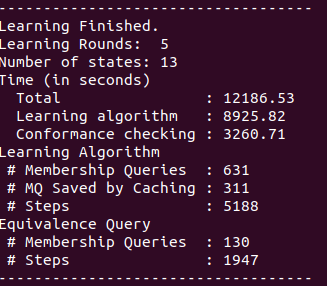
\includegraphics[width=\linewidth]{images/NoFilterA}
	\caption{Most common learned model.}
	\label{fig:nofiltera}
\end{figure}

In comparison, when learning the same server using retransmission-filtering, all non-deterministic behavior vanishes and we get the model shown in Figure \ref{fig:reference}. The model has only 6 states and therefore was learned much more quickly than the previous one, with learning requiring only 52 minutes (3098 seconds). Learning happened over two rounds, where the time was distributed more evenly between the learning algorithm and equivalence queries, with only roughly 60\% of the total runtime being used for the learning algorithm. 

\begin{figure}[h]
	\centering
	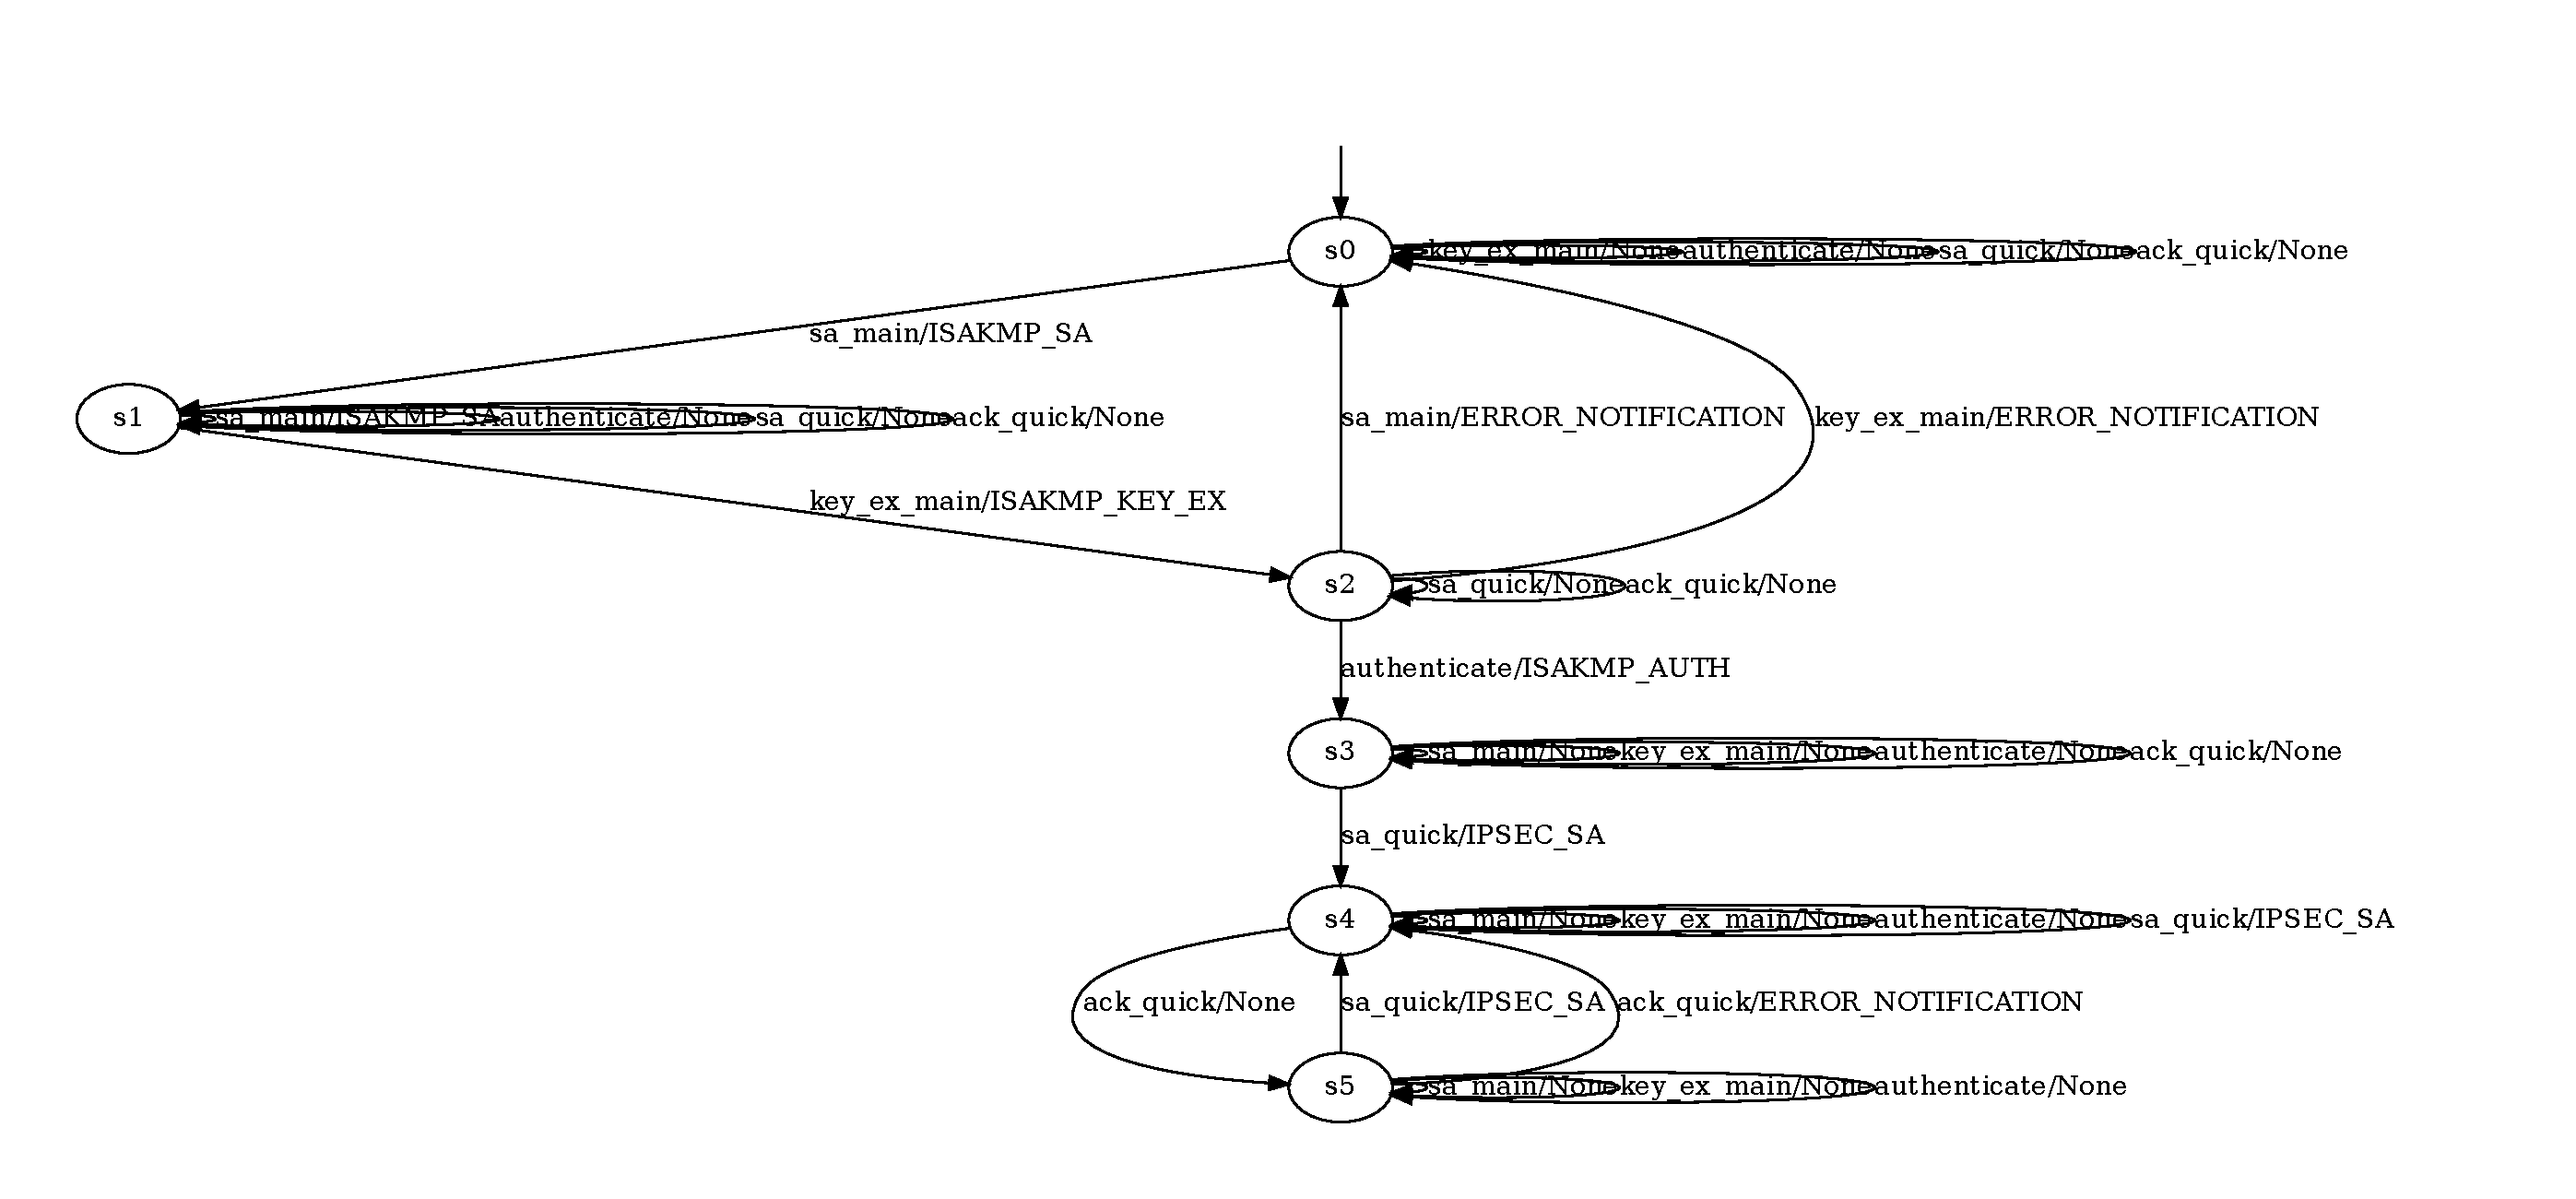
\includegraphics[width=\linewidth]{images/Reference}
	\caption{Clean model learned using retransmission filtering}
	\label{fig:reference}
\end{figure} 

Looking at the resulting model more closely, we can see that the first four states are identical to the previous model. This is due to the fact that the retransmissions only triggered for phase two messages and since they are our only source of non-determinism, we see no differences here. However, the phase two states look wildly different, showing a streamlined behavior that fits our reference IKE exchange (see Figure \ref{fig:IKEv1}) almost perfectly. The only small difference lies in the additional state \emph{S5} which loops back to state \emph{S4} with an \emph{IPSEC SA} or \emph{ACK} message. This behavior demonstrates how one can create multiple IPSEC SAs on a single IKE SA channel. And once a new IPSEC SA has been established, we can again send another \emph{ACK} message. In other words, the extra state is there to show that we cannot acknowledge a single IPSEC SA twice, but need to first create a new one.

% Error model
TODO: analyze error model
Figure \ref{fig:withfilterwitherrors} shows a model learned with retransmission-filtering enabled. Additionally, the input alphabet was expanded to include an additional erroneous version of each letter that maps to a malformed IKE message. This model served as the basis for our model-based fuzzing and was, thanks to the retransmission-filtering, 100\% deterministic. It took a total of 

TODO: rerun learning with Lstar alg, as runtime seems sus

The model looks largely identical to the previous model, apart from some additional self-transitions and one additional error transition from state \emph{S4} to \emph{S5}. Here, state \emph{S4} corresponds to the previous \emph{S6}. The error transition simply means that we need to create a valid IPSEC SA before we can acknowledge it.

\begin{figure}
	\centering
	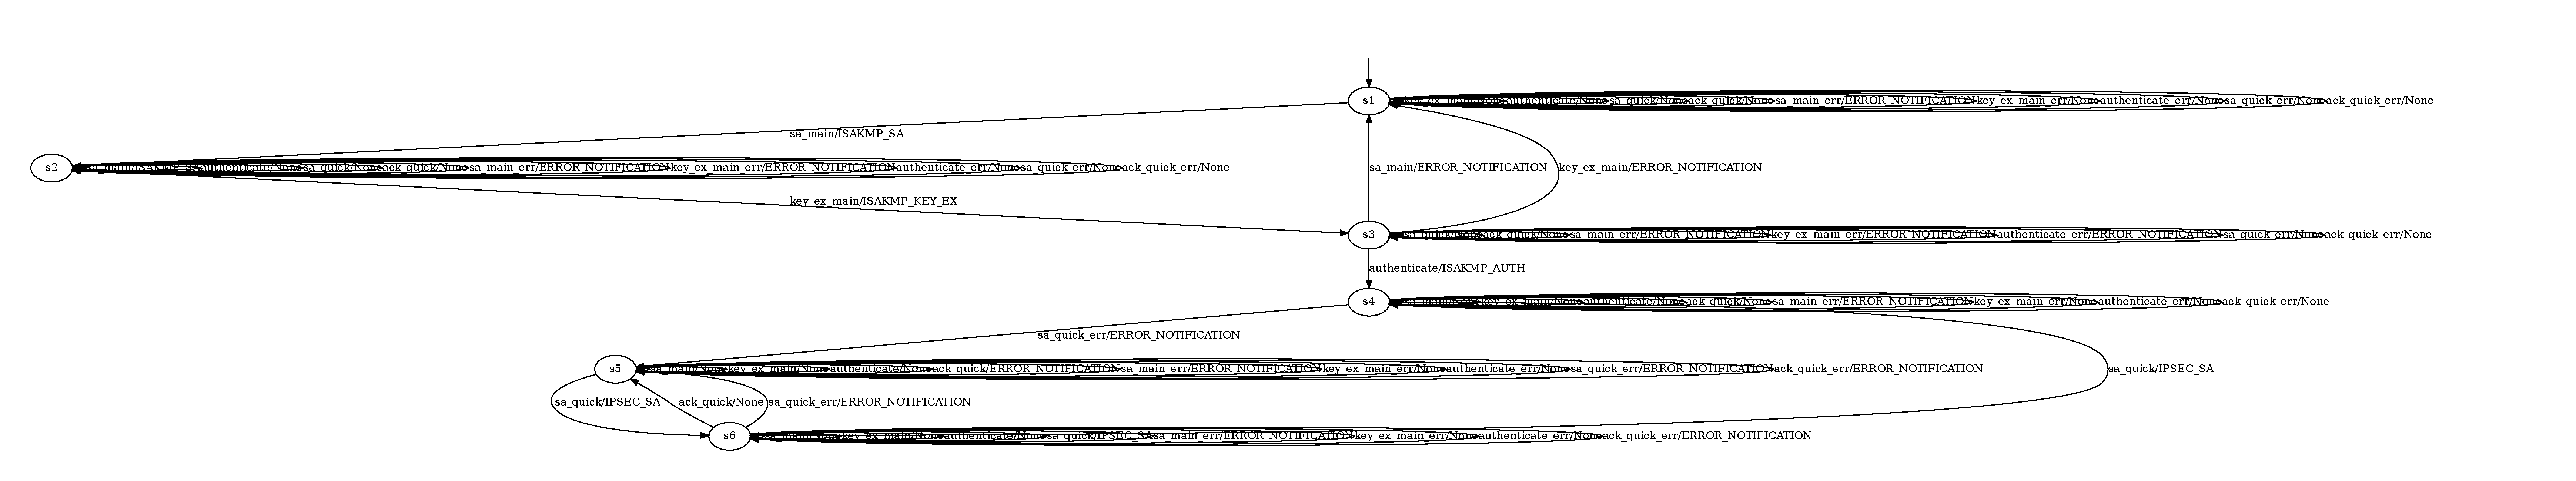
\includegraphics[width=\linewidth]{images/WithFilterWithErrors}
	\caption{Model with malformed messages}
	\label{fig:withfilterwitherrors}
\end{figure}

\subsection{Comparing $KV$ and $L^*$} \label{subsec:comp_kv_lstar}
% section copmaring KV and Lstar
TODO: Compare KV and Lstar


\subsection{Library Error} \label{subsec:liberror}
% section with discovered bug
TODO: Expand on this
faulty library fixes --> a persistent bug that even after several weeks of debugging. Initially we believed this to be caused by non-deterministic behavior of the SUL or problems in our code, but after comparing logs and packet captures, still occasionally would exhibit non-deterministic behavior and therefore crash. Bug appeared to occur randomly at different points during the learning process. Additionally, it did not occur consistently each learning attempt, which made debugging even more difficult. Finally we discovered a very niche bug in a used Diffie-Hellman python library where if the most significant byte was a zero, it would be omitted from the response, causing the local result to be different than the values calculated by the server. As this would only occur in the rare case where the MSB of the DH exchange was zero, this explains the random and difficult to reproduce behavior of the bug. As the library is not a very widespread one, the impact of this bug is presumably not all that high, still it might compromise the security of affected systems and the maintainer has been notified of the problem.

No way this bug would have been found with out the exhaustive testing done by the model learning procedure and without seeing the slight differences in the resulting models that did not crash during the learning process.
\section{Fuzzing Results} \label{subsec:fuzzresults}
test
% Two main parts, eval of learning and eval of testing